\chapter{Algebraic Curves}\label{chap2} %% chap2

Let\pageoriginale $K$ be an algebraically closed field. An
\textit{algebraic curve} 
over $K$ is a variety over $K$ all of whose irreducible components
have dimension $1$. In this chapter, we shall be mainly concerned with
irreducible complete, nonsingular curves. 

\section{The genus}\label{chap2:sec1}%sec .1

a) Let $C$ be a nonsingular curve. Then for any point $P \in C$, the
local ring $\mathscr{O}_{P}$ is a discrete valuation ring of the
function field $K(C)$. If, in addition, $C$ is complete, then every
discrete valuation ring of $K(C)$ dominates some $\mathscr{O}_P$,
$P\in C$ and hence equals that $\mathscr{O}_P$. Obviously the point
$P$ is uniquely determined. Thus the structure sheaf of a nonsingular,
complete, irreducible curve $C$ is determined by $K(C)$ and
any two birationally equivalent such curves are isomorphic. This fact
enables us to construct a projective ``model'' $C$ for a function field
of one variable $L$ ove $K$ in the following manner: 

Let $L = K(x_1,\ldots,x_n)$; consider any affine curve $C'$ in $K^{n}$
whose coordinate ring is $K[x_1,\ldots,x_n]$. We take for $C$ the
projective normalisation of a projective closure for $C'$. The curve
is normal (therefore nonsingular) complete, irreducible, with function
field $L$ and is thus the ``model'' we are looking for. 

But in the sequel, we need models of $L$ with ``nicer'' properties in
projective spaces of ``small'' dimension. We start with the following 

\begin{defi*}%defin
  $A$\pageoriginale nonsingular curve $C$ is said to be {\em strange} if all its
  tangents have a point in common, all if it is not a straight line. It is
  easily seen that strange curves can occur only in characteristic
  $p\neq 0$. 
\end{defi*}

\setcounter{theorem}{0}
\begin{theorem}\label{chap2:sec1:thm1}%them 1
  Any function field of one variable $L$ over $K$ admits:
  \begin{enumerate}[\rm i)]
  \item a nonsingular model, which is {\em not strange}, in $\mathbb{P}_3$.
  \item a model in $\mathbb{P}_2$ which has for its singularities only
    finitely many ordinary double points. 
  \end{enumerate}
\end{theorem}

\begin{proof}%proof
  We shall prove i) in two stages.
\end{proof}

\medskip
\noindent
{\bf {\boldmath $\alpha)~ L$} ~admits a nonsingular, nonstrange, projective model}.

\medskip
Let $C$ be a projective nonsingular model of $L$ in $\mathbb{P}_n$,
constructed as above. We may assume that $C$ is strange; choose a
system of homogeneous coordinates in $\mathbb{P}_n$, such that $C$
does not lie entirely in the hyperplane $X_o = 0$ and that $A =
(1,0,\ldots,0)$ is the common point of all the tangents of $C$. Let
the homogeneous coordinate functions on $C$ be $(1, x_1\ldots, x_n)$. 

Let $D$ be a nontrivial derivation of $L$ over $K$. For any point $P
\in C$, the parametric equations of the tangent $T_p $ to $C$ at $P$
are given by 
\begin{equation*}
X_i = \alpha x_i(P) + (Dx_i)(P), \alpha \in K, i = 0,\ldots, n.\tag{1}\label{chap2:sec1:eq1}
\end{equation*}

  The parameter ${\alpha_A}$ of $A$ on $T_{P}$ is a rational function of
  $P$, say $u\in L$. Thus, 
\begin{equation*}
  0 = ux{_i} + Dx{_i}  ~\text{for} i = 1,2,\ldots,n\tag{2}\label{chap2:sec1:eq2}
\end{equation*}
  and the system of homogeneous coordinates of $A$, given
  by (\ref{chap2:sec1:eq1})
  is\break 
  $(u,0,\ldots,0)$\pageoriginale whence $u\neq 0$. 

  We now claim that $\exists y \in L$ such that $uy + Dy$ is not
  proportional to $u$, i.e., such that $y + u^{-1}$ Dy $\in K$: in
  fact, as we are in characteristic $p \neq 0$, we may take any $y\in
  \text{L}^p-K$ (since $Dy =0$). Thus any model of $L$ for which the
  system of homogeneous coordinates is of the form  
\begin{equation*}
  (1,x_1\ldots,x_n,y,z_1\ldots,z_o),\quad  y,z_j \in
  L\tag{3}\label{chap2:sec1:eq3}
\end{equation*}
  is \textit{ nonstrange }. It remains to prove that there exists such
  a nonsingular model. 

Let $\mathcal{G}$ be a positive divisor on $C$ such that $(y)\geq -
\mathcal{G}$. Then $1$,$y$ $L(\mathcal{G})$ and $C$ being projective,
$L(\mathcal{G})$ is finite dimensional with a basis
$(1,y_1\ldots,y_r)$ with $y_1=y$. These then define a morphism
$\varphi_{\mathcal{G}}: C \rightarrow\mathbb{P}_r$ (Chapter I, \S
2) and as in Chapter I, \S 2. Proposition~\ref{chap1:sec2:prop3}, we get an
imbedding $\psi: C \xrightarrow{(1,\varphi\mathcal{G})} \mathbb{P}_n
\times \mathbb{P}_r \xrightarrow{\sigma}\mathbb{P}_{\text{nr+r+n}}$ of
$C$ in $\mathbb{P}_{\text{nr+r+n}}$. The homogeneous coordinate
functions on $\psi (C)$ are the functions $(x_i y_j)$ with $x_o = y_o
= 1$ and among then we have $1,x_1,\ldots,x_n, y;\psi(C)$ is
nonsingular and we have a model of type (\ref{chap2:sec1:eq3}). 

\medskip
\noindent
{\bf {\boldmath $\beta)$~ $L$}~ admits a nonsingular, nonstrange model in $\mathbb{P}_3$.}
\medskip

Let $C$ be a nonsingular, nonstrange model in some ${\mathbb{P}_n}$
(by $\alpha$)); let $n \geq 4$. The tangents $T$,$T'$ at two generic
points of $C$ do \textit{not} meet: otherwise any two tangents
meet. We recall here that an irreducible system of lines in
${\mathbb{P}_n}$ such that any two lines in the system meet, either is
a system of coplanar lines or has the property that all the lines of
system pass through a point. This then implies that $C$ is either\pageoriginale
planar or strange. Therefore the union $\begin{matrix}V
  \\ \lambda \end{matrix}$ of lines in ${\mathbb{P}_n}$ which meet $T$
and $T'$ has dimension $\leq 3$ in ${\mathbb{P}_n}$. 

We now consider the set of all chords $pp'$ in ${\mathbb{P}_n}$,
$P, P,'\in C$, $P$ \textit{not} necessarily distinct from $P'$ (thus,
the tangents to $C$ are also included); we claim that the union of
these chords forms an irreducible algebraic variety $W$ of dimension
$\leq 3$ in ${\mathbb{P}_n}$. In fact, let $k$ be a field of
definition for $C$, $(x)$ a generic point of $C/k,(x')$ a generic
point of $C/_{k(x)}$. Then the ``generic'' chord has the parametric
equations 
$$
{y_i = tx_{i} + (1-t)x_{i}'}.
$$

Taking $t$ transcendental over $k(x,x')$, the point $(y)$ is a generic
point over $k$ for the ``chord variety'', and our assertion is proved. 

We now take any point S in ${\mathbb{P}_n}$ \textit{not} in $V \cup W$
and project ${\mathbb{P}_n}$ into ${\mathbb{P}_3} $ with $S$ as the
vertex of projection. This projection $\pi $ is defined and injective
on $C$; also as $C$ is nonsingular the ``geometric tangent space'' is
the same as the ``Zariski tangent space'' for $C$ so that the mapping
induced by $\pi$ on the Zariski tangent space is also injective, which
means that the maximal ideal at $P \in C$ is generated by the maximal
ideal at $\pi(P) = P'\in \pi(C) = C'$. As $\pi$ is an injection on C
and on its Zariski tangent spaces, $\pi$ is \textit{birational} which
proves that $C$ is the normalisation of $\pi(C) = C'$.

\begin{minipage}{4cm}
\begin{figure}[H]
\centerline{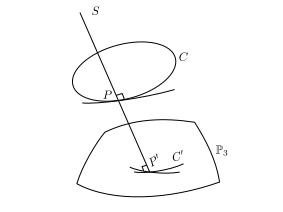
\includegraphics{vol36-figures/fig36-4.eps}}
\end{figure}
\end{minipage}\qquad  
\begin{minipage}{5.5cm}
  Now (by using the injectivity of $\pi$ again) one easily proves that
  ${\mathscr{O}_p}$is a finite ${\mathscr{O}_{P'}}$-module. As
  ${\mathscr{O}_{P'}\subset\mathscr{O}_P}$ and as both have the same
  residue field, viz, $K$, and as ${\mu_{P'},\mathscr{O}_P = \mu_{P}}$, by
  Nakayama's lemma we get ${\mathscr{O}_{P'} = \mathscr{O}_P}$. That is,
  $\pi$ is biregular. Therefore, $C'$ is nonsingular; in addition it is
  \textit{nonstrange}: in fact, as $S \notin V$, the projections $\pi (T)$
  and $\pi(T)'$ are tangents to $C'$ which do not meet. 
\end{minipage}
\bigskip
\pageoriginale

(ii) {\bf  $L$ admits a (birational) model in $\mathbb{P}_2$(K) with
  only modes as singular points.} 

Take a nonsingular nonstrange model $C$ of $L$ in $\mathbb{P}_3$
(by (i)). The tangents to $C$ form a variety of dimension 2 in
$\mathbb{P}_3$; and as $C$ is nonstrange the union of chords $PP'$ of
$C$ such that tangents to $C$ at $P$,$P'$ meet form a variety of
dimension $\leq 2$. Finally, the possibility that any chord $PP'$ is a
trisecant (i.e.meets $C$ at a third point) is ruled out as in that
case any two tangents to $C$ will have to meet; thus the union of
trisecants to $C$ forms a variety of dimension $\leq 2$ in
$\mathbb{P}_{3} (K)$. Therefore, choose a point $S \in\mathbb{P}_3
(K)$ avoiding: 

\begin{enumerate} 
\item [$\alpha)$] the surface of tangents to $C$
  
\item [$\beta)$] the trisecants to $C$
  
\item[$\gamma)$] the chords at whose ``extremities'' the tangents are
  coplanar. 
\end{enumerate}
 
Project\pageoriginale $\mathbb{P}_3(K)$ into   $\mathbb{P}_2(K)$ with $S$ as
vertex. $\gamma)$ and $\alpha)$ ensure that the projection is a
birational  map  $C$ onto its image $C'$. 

$\beta), \gamma)$ ensure that the
only singularities on $C'$ and ordi-nary double points. $C'$ is then
the require models in $\mathbb{P}_2 (K)$ \hfill {Q.E.D}

\textbf{b) The Riemann -Roch formula}
\medskip

A divisor $D$ on a nonsingular projective curve $C$ is a finite linear
combination, over  $\mathbb{Z}$, of points on $C, D  = \sum \limits _
{P \in   C}  n(P). P$, 
$n(P)=0$ for almost all $P \in C$. The \textit{degree} of $D= \sum
n(P).P$ is by definition $d (D)= \sum n(P)$. Any $x \in K (C)$ defines
a divisor $(x)=\sum \limits_{P  \in C} V_p (x), P, V_p$ being the
valuation of $K (C)$ defined by the local ring  $\mathscr{O}_P$ ; we
write $(x)=  (x)_\circ- (x)_\infty$  where  $(x)_\circ $ and
$(x)_\infty$ are both positive and are disjoint, the former defined by
the zeros of $x$ and  the latter by the poles. Elementary valuation
theory proves that $(x)_\circ, (x)_\infty$ have degrees equal to
$\big[K(C):K(x)\big]$. One deduces that $\deg (x)=0  \forall x  \in
K(C)$; thus one may talk of the degree of a  divisor class of $C$. 
 
For any divisor $D$ on $C$, the $K$-space
 
\noindent
$L(D)=\{x  \in   K(C): (x)\geq - D \}= \Gamma ( C, \mathscr{L}_D)$ is
finite dimensional (as $C$ is projective), say of dimension $l
(D)$. Then we have the following 

\setcounter{theorem}{0}
\begin{theorem}\label{chap2:sec1:thm1roch}{\rm (Riemann-Roch) (Preliminary form). }%them 1
  There exists an integer $g \geq 0$ and a divisor $\Omega$ on $C$
  such that\pageoriginale for any divisor $D$ on $C$ the following equality holds: 
  $$
  {l (D) = d (D)-g+1+l (\Omega- D)}
  $$
  We shall assume the theorem in this (a proof can be found in Serre
  \cite{7} Ch. The, 1.4, or in Chevalley \cite{1} Ch. II. \S 5,
  Th. 3). 
\end{theorem}

\medskip
\noindent\textbf{Consequences of the theorem}

\begin{enumerate}[(i)]
\item The integer $g$ is uniquely determined by the  above property.

  In fact, let $\Omega'$, $g'$ be another pair for which the above
  assertion holds. Take a divisor $D$ on $C$ such that $d(D)> d
  (\Omega)$  and  $d(D)> d(\Omega')$; then for this $D$, $l (\Omega-D)=0=
  l (\Omega' -D)$ and one obtains 
  $$ 
  g=g'={d(D)- l(D)+ 1}.
  $$
\item $ g=l (\Omega)$, and $ 2g-2=d (\Omega)$ as one sees by writing
  $D=0$ and $D= \Omega$ in the equality. 
\end{enumerate}

\begin{prop*}%propo
  Upto a linear equivalence the divisor $\Omega$ is uniquely
  determined by the properties: $l(\Omega) \geq g$ and 
  $$
  d (\Omega)= (2g-2).
  $$
\end{prop*}

In fact, suppose $\Omega'$ is a divisor on $C$ such that $ d
(\Omega')=2g-2$ and  $l(\Omega') \geq g$; then 
$$ 
\displaylines{\hfill 
  g \leq (2g-2)-g+1+l (\Omega-\Omega') \hfill \cr
  \text{i. e.,} \hfill l(\Omega-\Omega')\geq 1; \hfill }
$$
on\pageoriginale the other hand, $d(\Omega-\Omega')=0$.

The former implies that $\exists$ an $ x \neq 0 $ in $ K (C)$ such
that $(x)\geq (\Omega'- \Omega)$; but we know that $d ((x)),=0$; it
follows that  $(x)= \Omega'-\Omega$ and $\Omega'\sim  \Omega$. 

\begin{remark*}% rema
  The integer $g$ occurring in the Riemann-Roch Theorem is\break called the
  {\em genus} of the curve $C$; it can be defined for {\em any}
  irreducible curve and in fact for {\em any} function $L$ of one
  variable over $K$; by definition it is the genus of any projective
  nonsingular model $C$ for $L$. 
\end{remark*}

\begin{theorem}\label{chap2:sec1:thm2roch}%them 2.
  Let $C$ be any irreducible curve of degree $d$ in $\mathbb{P}_2
  (K)$. Then the genus $g$ of $C$ is given by 
  $$
  g= \frac{(d-1)(d-2)} {2}- \sum _{P  \in   C}  \dim_K
  (\mathscr{O}'_P/_{\mathscr{O}_p}) 
  $$
  where $ \mathscr{O}'_P$ is the integral closure of $\mathscr{O}_P$.
\end{theorem}

\begin{proof} %proof
  Choose a system of affine coordinates $x,y$ for $C$ such that  $C$
  has $d$ distinct points of intersection with the line at $\infty$
  and the affine equation for $C$ is of the form $F(x,y)=0, F$ a
  polynomial of degree $d$. The $d$ distinct points of $C$ at $\infty$
  define a positive divisor $D$ on $C$, of degree $d$. If $A$ is the
  affine coordinate ring of $C$ and $A'$ its integral closure, one has
  the equality 
  $$
  A'= \bigcup_{n \geq 0} L (nD);
  $$ 
  
  (Recall that for $ u \in K (C), P \in C, P $ is \textit{ not } a
  pole of $u  \Longleftrightarrow u$ is integral on
  $\mathscr{O}_p$). 
\end{proof}
 
Denote\pageoriginale $L (nD)$ by $ A'_n$;  and  $A'_n \cap A$ by $A_n$.  As $A'$ is
the integral closure of $A, \exists~ z \neq 0 $in $A$ such  that $zA'
\subset A$. 

Therefore $\dim_K (A'/A)= \dim_K \left(\dfrac{zA'} {zA}\right) \leq \dim
\left(\dfrac{A} {zA}\right)< \infty$. 

(A has Krull-dimension 1 and therefore $A/ _{ZA}$ Krull dimension 0,
this means that $A / \sqrt{zA} $is a finite direct product of
copies of $K$.)  It follows that  
$(\dim_K\mathscr{O}'_P/ \mathscr{O}_P) <\infty $  for all finite $P$;
and this is  trivial for $P$ at infinity so that $ \sum\limits _{P \in
  C}   \dim_K (\mathscr{O}'_P/ \mathscr{O}_P)$is a well defined
integer, and is equal to $ \dim_K (A'/A)$ by the properties of
localization of the integral closure.  

On the other hand $ A'_{n/A_n}= A'_{n/A'_n}\cap A$ is contained in $
A'/_A$;  as, from above, $ \dim_K (A'/_A)< \infty $ and as  $(A'_n)$
is an  increasing family it follows that, for large $n$ one must have
$ A'_{n/A_n}= A'/A$  and hence the equality 
$$ 
\dim_K A'_n= \dim_K A_n+ \dim_K (A'/ _A).
$$

Now $A_n$ consists of the classes modulo $F$ of polynomials $ f \in\break K
[X,Y]$ such that $d \circ f \leq n$; thus 

$\begin{aligned}
\dim_K A_n &= \frac{1}{2} (n+1) (n+2)- \frac{1} {2} (n-d+1) (n-d+2) \\
& =  nd+1 - \frac{1}{2} (d-1) (d-2). 
\end{aligned}$

Now applying the Riemann-Roch formula to the divisor $nD$, for large n
we obtain\pageoriginale $ nd+ 1 - \frac{1}{2} (d-1) (d-2)+ \dim_K (A'/_A) =nd-g+1+0$ 

$\begin{aligned}
\text{i.e.,}\qquad g & = \frac{1}{2} (d-1)(d-2)- \dim_K (A'/A)\\
&= \frac{1}{2}(d-1)(d-2)- \sum_{P \in C} \dim_K (\mathscr{O}'_{P/\mathscr{O}_P}) 
\end{aligned}$ \hfill Q.E.D

\begin{examples*}%exam
~

  \begin{enumerate}
  \item[(i)]  If $C$ is nonsingular of degree $d$ in $\mathbb{P}_2
    (K)$, then the genus of $C=  \dfrac{(d-1) (d-2)} {2}$. 
  \item[(ii)] Let $P$ be $a$ node on $C$.
  \end{enumerate}

  Choose a system of affine coordinates $(x,y)$ on $C_\lambda$ such
  that $P$ is the point  $(0,0)$.  Then $C$ is given at $P$ by an
  equation of the form $ 0= (F \equiv(ax^2+bxy+cy^2) +(\text{terms of
    degree } \geq 3)$; by hypothesis the square terms do not form a
  perfect square and the tangents at $P$ are given by $2ax+by=0,
  bx+2cy=0$; these are linearly independent and the maximal ideal at
  $P$ is given by 
  $$
  \mu = (x y)= (F'_x, F'_y).
  $$
\end{examples*} 

One can show easily that the integral closure $\mathscr{O}'$ of
$\mathscr{O} =\mathscr{O}_p $ satisfies the relation $F'_x
\mathscr{O}' \subset \mathscr{O}, F'_y \mathscr{O}'
\subset\mathscr{O}$, hence $\mu \mathscr{O}' \subset
\mathscr{O}$ and $x \mathscr{O} ' \subset \mathscr{O}$; we then
have  $   \mathscr{O} \supset x \mathscr{O} ' \supset x \mathscr{O}$;
as $\dim_K (\mathscr{O}/_{x \mathscr{O}})=2$ and 
$\dim_K  (\mathscr{O}/x \mathscr{O}')\geq 1$, 
it follows that $\dim_K \left(\frac{\mathscr{O}'}{\mathscr{O}}\right)
= \dim_K \left(\dfrac {x 
  \mathscr{O}'} {x \mathscr{O}}\right)=1$. Thus the contribution to
the sum   
$ \sum \limits_{P \in C}  \dim_K  (\mathscr{O}'_P/ \mathscr{O}_P)$
from a node $1$. In particular,if C is an an irreducible plane curve,
wish r nodes on it as the only singularities, and of degree $d$, then
the  genus $g$ of $C$ is   $ \dfrac{(d-1) (d-2)} {2}-r$. 

\section{Differentials on an curve}\label{chap2:sec2}%sec 2

Let\pageoriginale $A$ be a $K$-algebra. Then there is an $A$-module $\Omega
_{A/K}$ which is universal for $K$-derivations of $A$ in an
$A$-module. It is called the $A$- module of $K$-differentials  of
$A$. If $A$ is of finite type as a $K$-algebra,then $\Omega _{A/K}$ is
a finite $A$-module;  if $d; A \rightarrow \Omega _{A/K}$ is the
structural derivation then   $\Omega _{A/K}$ is generated over $A$ by
elements $   dx_\alpha, (x_\alpha)$ being a system of $K$- generators
of $A$. 

If $C$ is an algebraic curve over $K$  then $ \Omega_{K(C)/K} \text{
  is a } K(C)$  module; if  $x\in K(C)$ is a separating base of
$K(C)/K$ then $\Omega_{K(C)/K}$ has a base $(dx)$. 

One may also define a sheaf $\Omega$ of differentials on the curve $C$
(more generally, on any variety); this is defined by the presheaf $U
\longmapsto  \Omega_{A u/K}  $ on affine open sets $U$ with affine
algebra $A_U$; the stalk $\Omega_P$ of $\Omega$ at a point $ P \in
C$ is given by $\Omega _{\mathscr{O}_{P/K}}$.  The sheaf $\Omega$ is
locally free of rank $1$ on $\mathscr{O}$  and hence is a \textit{
  line bundle } denoted by $T^*(C)$, and called  the \textit{
  cotangent bundle} on $C$; it is the dual of the tangent bundle on
$C$ as is shown by the duality between  derivations and
differentials. An $  \omega \in \Omega _{K(C)/K}$is called a \textit{
  rational differential} on $C$. 

To any such differential $\omega$  on $C$ we associate a divisor
$(\omega)$ on $C$ in the following manner: at any point. $ P \in C,
\omega$  is of  the form $x$. dt, $x \in K(C)$   and $t$ a
uniformising parameter $P$; since $t-t(Q)$ is a uniformising parameter
at all $Q$ close to $P, \omega= x~ dt$ in\pageoriginale a neighbourhood of  
$P$ and we set $(\omega)= \sum  v_p  (x).P$ in this neighbourhood. It can be
shown that this expression is independent of the choice of $t$ so that
we obtain a divisor $(\omega)$ on $C,(\omega) =  \sum \limits _P v_P
(\omega).P$. 

\setcounter{proposition}{0}
\begin{proposition}\label{chap2:sec2:prop1} %propo 1.
  Let $C'$ be a model in $\mathbb{P}_2 (K)$ for $C$, of degree $d$,
  such that the only singularities of $C'$ are nodes. Choose a  system
  of affine coordinates $(x,y)$ in $ 2^{(K)}$  such that $C'$ has
  affine equation $F(x,y) =0$ and all the nodes are at finite
  distance; assume also that  the points $x=0,y=0$ on the line at
  $\infty$ are not on $C'$. Let $T$ be a polynomial in two  variables
  such  that the  curve $T(x,y)=0$ passes through all the nodes on
  $C'$. Then the differential  
  $$ 
  \omega= \frac{T (x,y)dx} {F'_y}= \frac{T(x,y)dy} {F'_x}
  $$
  on $C'$ (i.e. of $K(C'$)) defines a differential $\omega$ on $C$
  with the property that $(\omega)  \geq 0$ at all points $P$ at
  finite distance on $C$; if, in addition, $  d^\circ T \leq (d-3)$
  then $(\omega) \geq 0 $ on $C$ (we may say in this case that
  $\omega$ is \textit{ regular } or is of the\textit{ $1^{st}$ kind on
    $C$)}. 
\end{proposition}

\begin{proof}%proof
  \begin{case}\label{chap2:sec2:case1}
    Let $P$ be a simply point on $C'$. Then $ F'_x \neq 0$ or  $F'_y
    \neq 0 $ at $P$ and correspondingly $y$ or $x$ will serve as a
    uniformiser  at  $P$.Then $  v_p (\omega)= v_p (T) \geq 0$. 
  \end{case}
  \begin{case}\label{chap2:sec2:case2}
    By\pageoriginale hypothesis, $ T \in (F'_x ,F'_y)$ (\S 1,  Ch II) this proves
    that $v_P (\omega)\geq 0$ for every branch of a node; moreover if
    $T=0$ passes through the nodes in a ``nice'' manner (i,e
    transversal to both the  branches of $C'$ at any node) $ T/F'_x $
    and $T/F'_y $ will be with invertible  on each at  any node,  and
    $v_P (\omega)$ (which , in any case will be $\geq 0$) becomes
    zero. 
  \end{case}
  \begin{case}\label{chap2:sec2:case3}
    If $P$ is at $\infty$ on $ C'$, (by our choice of coordinates) we
    may take $z=\dfrac{1} {x}$ to be a uniformiser at $P$ ; then
    $\omega $ takes the form $\dfrac {-T} {F'_y} \dfrac {dz}{z^2}$ and 
  \end{case}
    \begin{align*}
      v_P(\omega) & = (-\deg.  T-2 + (d-1))\\
      & = d-3- d^\circ T;
    \end{align*}
    if $d^\circ T \leq (d-3)$, this means that  $v_P (\omega)
    \geq 0 $ for $P$ at $\infty$. \hfill{$ Q.E.D$.}
\end{proof}

\subsubsection*{Consequences of Proposition 1.}

\begin{corollary}\label{chap2:sec2:coro1}%cor 1
  The differentials $\omega$ of the first kind on $C$ form a $K$-
  space of dimension $\geq g$, the genus of $C$. 
\end{corollary}

By Proposition~\ref{chap2:sec2:prop1}, case (\ref{chap2:sec2:case3}), the space of regular differentials
on $C$ is of dimension $\geq \dfrac {(d-3+1) (d-3+2)} {2}-r$, where
$d$ is the degree of the plane model $C'$ of $C$  and $r$ its number
of nodes; the number on the right hand side is precisely the genus $g$
of $C'$, hence of $C$. 

\begin{corollary}\label{chap2:sec2:coro2}%coroll 2
  For\pageoriginale any differential $\omega$ in $C$, $d((\omega)) =  2 g -2$. As
  $\omega_{K(0)/K}$ is 
  one dimensional ove $K(C)$ and as $d ((f))= 0  \forall f \in K(C)$,
  we may take $\omega$ to be of the form $\dfrac{ T ~dx}{F_y}$ as in the
  proposition~\ref{chap2:sec2:prop1} with $T$ such that $T(x,y)=0$ passes through the
  nodes on the plane model $C'$ of $C$ in a ``nice'' manner and does
  {\em not} pass through any point on $C'$ at $\infty$. 
\end{corollary}

Thus we have, on the one hand 
$$
d ((\omega))= \underset{\substack{ P ~\text{finite}\\  \text{simple on}
    C^\prime }}{\sum} v_P (T) +d (d-3 -d^o T)  
$$
and on te  other hand
\begin{align*}
  (T \cdot C') & = d\cdot (d^o T)\\
  & = \underset{\substack{ P  ~\text{finite}\\  \text{simple on} C^\prime
  }}{\sum} v_P (T)+2r 
\end{align*}

$\begin{aligned}
  \text{ Thus },\quad d((\omega)) & = d \cdot (d^o T)- 2r+d  (d-3 - d^o T)\\
  & = -2r+d(d-3)\\
  & =  {2g-2}.
\end{aligned}$ \hfill Q.E.D

Let $C$ be a nonsingular, complete  irreducible curve and $\omega$ a
differential on $C$. Then the divisor $(\omega)$ defined by has the
properties $l ((\omega )) \geq g$ (by Cor. $1$ to
Proposition~\ref{chap2:sec2:prop1}:
$(f) \geq - (\omega) \Longleftrightarrow (f \omega) \geq 0), \text{
  and } d (( \omega)) = (2g-2) (Cor.2)$. Thus,\pageoriginale as we have seen before
(niemann-Roch, preliminary form)  the divisor class $  \Omega \text{
  of } (\omega)$ satisfies 

\begin{theorem*}[ (Riemann Roch-Final form)]%them 
  For any divisor $D$ on $C$, one has the equality
  $$ 
  l(D) = d(D)- g+1+l (\Omega-D).
  $$
  
  As $\Omega_{K(C)/K}$ is one -dimensional over $K(C)$, it follows
  that $\Omega$ \textit{is the class of all differentials} on  $C$; we
  call it the \textit{canonical class} on $C$. 
\end{theorem*}

\section{Projective Imbeddings of a curve}\label{chap2:sec3}%sec 3

Let $C$  be a  complete, nonsingular irreducible curve and $D$  a
divisor on $C$. Let $(f_o,\ldots,f_n)$ be a basis for $L(D)$; as
before, they define a morphism $\varphi =\varphi_D $ from $C$ to
$\mathbb{P}_n $(K). 
\begin{enumerate}
\item [(i)] Assume that $P$ is a point on $C$ with $ L(D)
  \underset{\neq} \supset L(D-P) \underset{\neq} \supset L(D-2P)$. 

  Then $\mathscr{O}_{\varphi _(P)}$ contains a uniformising parameter
  for $\mathscr{O}_p$. 

  In fact, if $ x \in L (D)-L (D-P)$, and  $y \in L(D-P)-L (D-2P)$
  and $z= y/x$ then $z \in \mathscr{O}_{\varphi (P)}$ and $v_P (z)=v_P
  (y)-v_P(x)$ 
  $$
  = v_P (-D)+1-v_P (-D)=1.
  $$
\item[(ii)] Assume that $P,P'\in C$ such that
  $$
  L(D)\underset{\neq}{\supset} L(D-P-P)\underset{\neq}{\supset} L(D-P-P').
  $$
  %%%\varsupsetneqq
  Then $ \varphi (P)\neq \varphi (P')$.
\end{enumerate}

Let\pageoriginale $\lambda \in L(D) - L(D-P)$ and $y \in L(D-P) - L(D-P-P')$, and
$u=y/x$; then $u$ defines a function $\tilde{u}$ on the image in a
natural way. And $\tilde{u} (\varphi (P'))= u(P') = 0 $ while
$\tilde{u} (\varphi (P'))= u(P') \ne $ so that $\varphi({ P)
  \ne(P')}$. 

\begin{theorem*}%them
  For a divisor $D$ on $C$ with deg. $D \geq 2g+1$
  $\varphi_{D}$ is an imbedding.	 
\end{theorem*}	

\begin{proof}%proof
  For $P,P' \in C$ one has $d(D-P)$ $\geq 2g$ and $d(D-2P) =
  d(D-P-P')$ $\geq$ $2g-1 > (2g-2)$ so that by the Riemann-Roch
  formula 
  \begin{align*}
    & l ( D) = d(D) - g + 1 \geq g+2\\
    & l ( D-P) = l(D) - 1 \geq g+1\\
    & l ( D-P-P') = l(D) - 2 = 1(D-2P) \geq g
  \end{align*}	
  and one obtains:
  \begin{align*}
    & L( D)\underset{\neq}{\supset} L(D-P) \underset{\neq}{\supset}
    L(D-2P)\\ 
    & L( D)\underset{\neq}{\supset} L(D-P) \underset{\neq}{\supset}
    L(D-P-P'). 
  \end{align*}
\end{proof}

By (i) preceding the theorem, $\varphi_{ D}$ is an unramified morphism
and by (ii) it is injective. As $C$ is nonsingular, one proves that
$\varphi_{ D}$ is an imbedding as in \S 1. \hfill Q.E.D

\begin{examples*}
~

  \begin{enumerate}
  \item[(i)] $g = 0$, 1: classical line, cubic curve.
  \item[(ii)] $g \ge 2$: the divisor $D = 3 \Omega $ satisfies $d(D)
    \ge  2g + 1$ and thus defines an imbedding $\varphi_{ D}$ {\em
      (the Tricanonical imbedding)}. 
  \item[(iii)] on (any nonsingular) $C$, {\em any positive divisor is ample}.
  \end{enumerate}	
\end{examples*}	

\section{Morphisms of algebraic curves}\label{chap2:sec4}%sec 4

(a)~\pageoriginale Let $C$ be a nonsingular, irreducible complete curve and $\Delta$
the diagonal in $C \times C$. Then ``self-inter section'' $\Delta
\cdot\Delta$ is a divisor class on $\Delta$ defined in the following
manner; let $\varphi$ be a function on $C \times C$ such $v_\Delta$
($\varphi )= 1$; then $\Delta . (\Delta - (\varphi '))$ is
well-defined on $\Delta$ ; if $\varphi'$ is any other function on $C
\times C $ such that $v_\Delta$ ($\varphi')= 1 $ then
$\varphi'/_\varphi$ can be restricted to a regular function $\theta$
on $\Delta$ and one has 
$$
\Delta \cdot (\Delta -(\varphi )) - \Delta \cdot (\Delta - (\varphi' )) =
\Delta\cdot\big(\frac{\varphi'}{\varphi}\big)=(\theta) 
$$	
so that the class of $\Delta\cdot(\Delta - (\varphi ))$ is independent of
the choice of $\varphi$; call it $\Delta , \Delta$. We have the  
\begin{theorem*}%them 
  $\Delta \cdot \Delta = -\Omega_\Delta$, the class on $\Delta$ defined by
  the canonical class $\Omega$ on $C$; therefore, the intersection
  number ($\Delta \cdot \Delta$) is $(2 - 2g)$. 
\end{theorem*}

\begin{proof}% proof
  Take a separating function $f \in K(C)$; then $df \ne 0$. Define
  $\varphi$ on $C \times C $ as $\varphi(P,Q) = f(P) - f(Q)$. One has
  clearly $v_\Delta(\varphi)=1$. 

\medskip
  \begin{minipage}{5.5cm}
    \begin{figure}[H]
      \centerline{\includegraphics{vol36-figures/fig36-5.eps}}
    \end{figure}
  \end{minipage}\quad 
  \begin{minipage}{4cm}
    Also, if $f= {\sum\limits_{n \ge n_o}
      a_n u^n}$ is the Taylor expansion of $f$ at a point $P$ on $C$,
    then $\varphi$ is locally given by $\varphi = \sum a_n (u^n - v^n)$
    on $C \times C $ ; the local equation of $(\varphi)-\Delta$
    is thus $\sum\limits_{n \geq n_\circ} a_n \frac{u^n - v^n}{u-v}$;
    from this one deduces by an easy computation that the local
    education of 
  \end{minipage}
\medskip  

\noindent $pr (\Delta \cdot ((\varphi) -\Delta))$ is 
  $ {\sum\limits_{n \geq n_o} na_n u^{n-1} = \dfrac{df}{du}}$\pageoriginale
  and the coefficient of $(P,P)$ in $\Delta \cdot ((\varphi )- \Delta)$ is
  therefore $v_ p (df)$. \phantom{WWWWWWWWWW}\hfill Q.E.D.
\end{proof}

\begin{coro*}%coroll
  Let $f \in K(C)$; if $\varphi \in K(C \times C)$ is given by
  $\varphi(P,Q) = f(P) - f(Q)$, then the divisor $\Delta .(\Delta -
  (\varphi))$ on $\Delta$ in $C \times  C$ is given by $-(df)_\Delta
  $. 
\end{coro*}	
	
(b) Let $C,C'$ be nonsingular, irreducible, complete curves and $\pi :
C \rightarrow C'$ a morphism; let $\pi^* : K(C')\rightarrow K(C)$ be
the cohomomorphism of $\pi$. For any $P' \in  C'$, the discrete
valuation $v_{ P'}$ with centre $P'$ of $K(C')$ extends to discrete
valuations $v_{P_1} ,\ldots , v_{P_r}$ of $K(C)$ with centres $P_1 ,
\ldots , P_r $; we thus define a divisor $\pi^*(P') =
\sum\limits_{i=1}^{r} e_i P_i$ where $e_ i$ is the ramification index
of the extension $v_{P_i}$ over $v_{P'}$. The degree of $\pi^*(P')$ is
then equal to $\sum\limits_{i=1}^r e_i = n = \big[K(C) :
  K(C')\big]$. The definition is extended by linearity to all divisors
on $C'$. We say that $\pi$ is \textit{unramified} if all the $e_i$ are
$1$. If $(f'), f' \in  K(C')$, is a principal divisor on $C'$,
$\pi^*((f'))$ is principal on $C$ defined by $ \pi^* f' \in K (C)$. If
$\pi$ is separable (i.e. if $K(C)/K(C')$ is separable) and $\omega'
=x' dt'$ is a differential on $C'$, then $\pi^*(\omega')=\pi^*{ x'
  .d(\pi^*t')}$ is a differential on C; and for any $z' \in K(C'),
{\pi^*(z'\omega')=\pi^*z'. \pi^*(\omega').}$ We shall now prove a
theorem which shows how $\pi^*((\omega'))$ and $(\pi^*(\omega'))$ are
related on $C$. 

\begin{theorem*}[ (Hurwitz-Zenthem)]%them 
  If\pageoriginale $\pi$ is a separable morphism $C \rightarrow C'$, then for any
  differential $\omega'$ on $C'$ 
  $$ 
  (\pi^\ast (\omega')) - \pi^\ast (\omega') = \underline{d} 
  $$
  where $\underline{d}$ is the different of $K(C)/{K(C')}$.
\end{theorem*}

\begin{proof}%proof
  Let $P \in C$ and $P'= \pi(P)\in C', z$ a uniformising parameter at
  $P'$, $t$ a uniformising parameter at $P$. We have $\mathscr{O}=
  \mathscr{O}_{ p} { \supset \mathscr{O}_{P'}}=\mathscr{O'}$ and
  $K[[t]] = \hat{\mathscr{O}} \supset \hat{\mathscr{O'}} = K[[Z]]$ and
  finally $\widehat{\mathscr{O}} = \widehat{\mathscr{O'}} [t]$. One
  has an exact sequence of $\hat{\mathscr{O}}$-modules 
  
  $\Omega_{\hat{\mathscr{O'}}/{ K}}\otimes \hat{\mathscr{O}}
  \rightarrow \Omega_{\hat{\mathscr{O}}/ K} \rightarrow
  \Omega_{\hat{\mathscr{O}}/\hat{\mathscr{O'}}}\rightarrow 0$. 
\end{proof}

Thus $\Omega_{\hat{\mathscr{O}}/\hat{\mathscr{O}}}$  is identified
to the quotient of $\Omega_{\hat{\mathscr{O}}/ K}$ by $dF$ where
$F$ is the minimal polynomial of $t$ over $\mathscr{O}'$. Identifying
$\Omega_{\hat{\mathscr{O}}/K}$ with
$\hat{\mathscr{O}}$, thanks to the base $dt$, one finds that
$\Omega_{\hat{\mathscr{O}}/\hat{\mathscr{O}}}$ is identified with
$\hat{\mathscr{O}}/_{(F'(t))}$. The different of $\hat{\mathscr{O}}
/_{\hat{\mathscr{O}'}}$ is thus generated by $(F'(t))$. 
		
Now, we first observe that $(\pi^*(\omega')) - \pi^* ((\omega'))$ is
independent of $\omega'$; thus, set $\omega' =dz$. Then $v_{
  P'}(\Omega')=0$; and therefore if $dz=y dt$ one obtains 
$$
\displaylines{\hfill 
  v_P(dz)  = v_{P'}(\pi^* (\omega' ))=v_P(y) =v_P(F'(t))\hfill \cr 
  \text{and}\hfill v_P ((\pi^*(\omega' )) - \pi^* ((\omega' ))) =
  v_P(F'(t))  -v_{P'}(\omega') =v_P(d)-0.\hfill}
$$ 

One\pageoriginale deduces then that 
$$
(\pi^* (\omega' )) -\pi^* ((\omega' ))= { d.}.
$$
\hfill Q.E.D.

\noindent \textbf{Corollaries. }
  Let $g$ and $g'$ be the genera of $C$ and $C'$.
  \begin{enumerate}[(i)]
  \item By the above theorem we obtain
    $$
    2g - 2 - n(2g' - 2) = d^\circ(d) \ge 0.
    $$
  \item \textit{Luroth's theorem.}
    
    \textit{If $g = 0$ then $g' = 0$.}
    
    From (i), we obtain for $g=0$,
    \begin{align*}
      { - 2 - n(2g' - 2)}& \geq 0\\
      { n(2g' - 2)}  & \leq -2
    \end{align*} 
    which implies that $g' = 0$.
  \item $g' = 0, \pi $ unramified $\Rightarrow n = 1, g = 0$.

    Note that $\pi$ unramified $\Leftrightarrow d = 0$ so that by (i),
    
    $2 - n (-2) = 0$ and $n = 1-g$ which implies $g = 0$, $n = 1$.
  \item \textit{$g = 1 \Rightarrow g' = 0, 1$}.

    By $(i)$, $-n(2g' - 2)\geq 0$, i.e. $g' = 0$ or $1$
  \item $g = 1$, $g' = 1 \Rightarrow \pi$ unramified
  \item $g' = 1, \pi$ unramified $\Rightarrow g = 1$.
  \end{enumerate}			

\textbf{(c)}~ Let $\pi : C \rightarrow C'$ be a separable morphism as in
$(b)$. Then the graph $T=(\pi \times \pi)^{-1}(\Delta')(\Delta' = $
diagonal in $C' \times C')$ of the equivalence relation defined by
$\pi$ on $C$ is a cycle on $C \times C$ in a natural\pageoriginale way. If $d$ is
the different of $K(C)/_{ K(C')}$ then one has  

\begin{theorem*}%them 
  $$
  \Delta. (T - \Delta) = (d)_\Delta 
  $$
\end{theorem*}

\begin{proof}%proof	
  Write $T = \Delta + S$. Then the set of all points $P_{ i}'$ in
  $\pi(pr_C(\Delta \cap S))$ is finite and one can find a function
  $f'$ on $C'$ which is a uniformiser at all $P_{ i}'s$. We define a
  function $u'$ on $C'\times C'$ by $u'(P',Q') = f'(P') -
  f'(Q')$. Then $v_{\Delta'}(u') = 1$ and $\Delta'.((u')-\Delta')=
  (df')_\Delta$ by the corollary to the theorem of $(a)$. We set $f=
  \pi^*f'$ and $u= \pi^*u'$ so that $u(P,Q) = f(P)-f(Q)$ on $C \times
  C$. Also, if $(u') = \Delta' + X'$ then $(u) = T+X$ with $\pi^{-1} =
  (X')=X$ and thus $(u) = \Delta + S + X$. One then deduces that  
\end{proof}

\begin{align*}
  (\Delta + S). X & = \pi^* (\Delta'\cdot X') = \pi^* (df')_\Delta\\
  &=  (df)_\Delta - d_\Delta \text{(by Hurwitz's theorem)}.
\end{align*}

On the other hand,
\begin{align*}
  (\Delta + S). X & = \Delta .((u) - \Delta - S) + S.X\\
  &=  (df)_\Delta - \Delta. S + S.X.
\end{align*}

Therefore,
$$
\Delta \cdot S - \underline{d}_\Delta = S.X.
$$

But if $P \in S. X$ then $\pi(P) = P' \in  S'. X'$ so that 
$$ 
P \in (S.X) \cap \Delta \Rightarrow P' \in (S'.X') \cap \Delta
$$
and $(df')(P') = 0$. But we have chosen $f'$ to be a uniformising
parameter at $P'\in \pi (pr_{C}(\Delta \cap S))$ and hence $(df')(P')$
cannot be zero. This\pageoriginale proves that $S.X$ as a cycle on $C \times C$,
disjoint from $\Delta$, and we deduce then from the last equality that  
$$
\displaylines{\hfill 
  S.X  = 0 \hfill \cr 
  \text{and}\hfill  \Delta .S  = \underline{d}_\Delta \hfill \cr
  \text{i.e.} \hfill d_\Delta  = \Delta.(T-\Delta)\hfill \text{Q.E.D.}}
$$
	
\begin{theorem*}[ (Schwarz-Klein)]%them 
  A curve $C$ of genus $\geq 2$ admits only finitely many automorphisms.
\end{theorem*}

\begin{proof}%proof
  Let $X$ be any cycle on the product $C \times C$. If $C_1$ and $C_2$
  are the ``horizontal'' and ``vertical'' in $C \times C$, one defines the
  {\em indices} of $X$ as the intersection numbers $(X.C_1) = d_1 $
  and $(X.C_2) =d_2$. If $C \times C \hookrightarrow \mathbb{P}_n$ is
    a projective imbedding of $C \times C $ and $X$ is a cycle of $\dim 1$
    on $C \times C$, then the projective degree of $X$ in $\mathbb{P}_{
      n}$ is completely determined by its indices $d_1$ and $d_2$ in $C
    \times C$ and the degree of $C \times C$ in $\mathbb{P}_{ n}$. 
    More precisely, consider an imbedding $C \hookrightarrow \mathbb{P}_{
      r}$ ; this defines an imbedding $C \times C \hookrightarrow
  \mathbb{P}_{ r} \times \mathbb{P}_{ r} \hookrightarrow \mathbb{P}_{
    r^2 + 2_r}$ and the homogeneous coordinates in the image are of
  the form $(z_{ ij}) = ( x_ i y_ j)$. 


  \begin{minipage}{5.5cm}
    \begin{figure}[H]
      \centerline{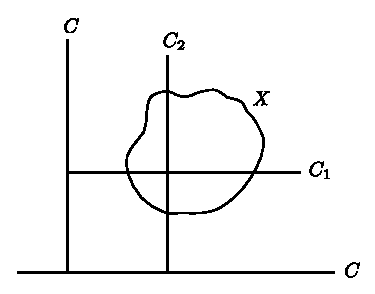
\includegraphics{vol36-figures/fig36-6.eps}}
    \end{figure}
  \end{minipage}\qquad 
  \begin{minipage}{4cm}
  Consider a hyperplane $H\equiv
  \sum\limits_{ i,j}{ a_j b_j z_{ij}}= 0$ in $\mathbb{P}_{ r^2 +
    2r}$, which is the product of two hyper planes $H_1 \equiv \sum 
    a_i x_i =0$ and $H_2 \equiv \sum_{b_j x_j} = 0$ in $\mathbb{P}_{ r}$. If
  the degree of $C$ in $\mathbb{P}_{ r}$ is $d$ and $d$ if $X$ is a cycle
  of inlices $d_1$ and $d_2$ in $C \times C$ then the intersection
  $H(C \times C)$ in $\mathbb{P}_{ r^2 + 2r}$ is given by  
  \end{minipage}
  \bigskip

  $$
  H(C \times C) = (H_1.C)\times C + C \times (H_2.C)
  $$
  so\pageoriginale that the intersection number $(H.X)$ is equal to $d(d_1 +
  d_2)$. Thus, the positive cycles of $\dim 1$  on $C \times C$ with
  given indices $d_1$ and $d_2$ form a finite union of irreducible
  algebraic families. (of Theory of  Chow coordinates). Now a positive
  cycle $T$ of dimension $1$ in $C \times C$ is the graph of an automorphism
  $\sigma$ of $C \Leftrightarrow T$ has indices $1,1$; it follows in
  particular that the graphs of automorphisms of $C$ form a finite
  union of irreducible algebraic families. We will be through,
  therefore, if we prove that every irreducible system of graphs of
  automorphisms of $C$ is of dimension $0$; let $(T_ \sigma)_\sigma$
  be such a system; if its dimension $\geq 1$, fixing an automorphism
  $\sigma_\circ$ of $C$, the system $(T_\sigma
  T_{\sigma_\circ}^{-1})_\sigma$ is irreducible, contains $\Delta$ and
  a $T \ne \Delta$ by assumption. We then have $(T.\Delta ) = (\Delta
  . \Delta)$. On the other hand, $(T. \Delta ) \ge 0 $ while $(\Delta
  . \Delta)= 2 - 2g < 0 $(note that $g \le 2)$. This contradiction
  proves our theorem. 
\end{proof}

\begin{coro*}%coroll
  Let $K$ be an algebraically closed field and $K'$ any extension of
  $K$. Let $L_1$ and $L_2$ be function fields of one variable over
  $K$, of genus $\ge 2$ and linearly disjoint from $K'$ over $K$.Then
  any $K'$-isomorphism $K'(L_1)\rightarrow K'(L_2)$ is the extension
  of a $K$-isomorphism $L_1 \rightarrow L_2$. 
\end{coro*}

\begin{proof}%proof
  Choose\pageoriginale a ``big'' algebraically closed $\Omega \supset K'$ models
  $C_1 $ and $C_2 $ for $K'(L_1)$ and $K'(L_2)$ over $\Omega$. We have
  bijections  
  \begin{align*}
    &\Big\{ \text{ $K'-$isomorphisms of $K'$} ~(L_1) ~\text{on}~
    K'(L_2) \Big\} \\ 
    \leftrightarrow & \Big\{ \text{ $K'-$isomorphisms of}~ C_2 ~\text{on}~ C_1
    \Big\} \\ 
    \leftrightarrow & \Big\{ \text{ $K'-$automorphisms of}~ C_1\Big\}.
  \end{align*}
  
  By hypothesis of linear disjointness, the genus of $C_1$ over the
  algebraic closure $\bar{K'}$ of $K'$ is $\ge 2$ and by the theorem
  of Schwarz-Klein the number of $K'$-automorphisms of $C_1$ is
  finite. 
		
  Consider any $K'$-isomorphisms $K' (L_1)\rightarrow K' (L_2)$. If
  $L_1 =\break K(x_{1,\ldots,}{ x_p})$ and $L_2 = K(y_{,\ldots,}{ y_q})$,
  this defines rational functions $R_{ i}$ and $S_{ j}$ over $K$ such
  that  
  \begin{align*}
    & \varphi(x_i) = R_i(y_{1,\ldots,}y_{q,} \lambda_1,\ldots, \lambda_s) \\
    & \varphi^{-1}(y_j) = S_j (x_{1,\ldots,}x_p, \lambda_{1,\ldots,}
    \lambda_s) \\ 
  \end{align*}	
  with the $\lambda's $ in $K'$. The locus of $( \lambda_1,\ldots,
  \lambda_s) \in \Omega^{ s}$ over $K$ is zero dimensional as each
  specialisation gives a $K'$-isomorphism. As $K$ is algebraically
  closed, one concludes that $(\lambda_1,\ldots, \lambda_ s)\in
  K^s$. The corollary is proved. 
\end{proof}

\begin{remark*}%rema
  This corollary shows that, if $C$ is a curve of genus $\ge 2$
  defined over an algebraically closed field $K$, then every
  automorphism of $C$ is defined over $K$. 
\end{remark*}
		
\begin{theorem*}[ (Severi)]%them
  Let $K$ be an algebraically closed field and $L$ a function field of
  one variable over $K$. Then the intermediary extensions $K
  \underset{\ne}{\subset} L' \subset L$\pageoriginale such that genus $L' \ge 2 $
  and $L/_{L'}$ is separable, are finitely many in number. 
\end{theorem*}

\begin{proof}%proof
  Let $C$ be a model for $L$ over $K$. any $L'$ with the given
  property, take any model $C'$ of $L'$ over $K$; the inclusion
  $L'\hookrightarrow L$ defines a morphism $\pi : C \rightarrow C'$ ;
  if genus $C= g$ and genus $C' = g'$; we have the equality $ 2g-2 = n
  (2g' - 2) + d^{\circ}(\underline{d})$ where $n=[K(C) : K(C')] = [L :
    L']$ and $\underline{d}$ is the different of $L$ over $L'$. As
  $d^\circ(d)\ge 0$ and $g$ is given, the number of choices for $g'\ge
  2$ and $n$ is \textit{finite. Thus we may assume that}  $n$ and $g'$
  \textit{are also given.} 
\end{proof}
			
Take then a curve $C'$ such that $K(C')$  is of genus $g'$ and $K(C)$
is separable of degree $n$ over $K(C')$. Consider the graph $T$ in $C
\times C $ of the equivalence relation defined by the morphism $\pi :
C \rightarrow C'$. Then $T$ is a cycle of dimension $1$ of the form
$T= \Delta + S$, symmetric about $\Delta$. 
			
$T$ can be considered as a correspondence of $C$ in $C$, i.e. as a
divisor on $C \times C$. Thus one can form the composite
correspondence $ToT$; more generally, if $A$ is a correspondence of
$C_1$ in $C_2$ and $B$ is a correspondence of $C_2$ in $C_3$, the
composite correspondence $AoB$ of $C_1$ in $C_3$ is defined by  
$$
AoB = pr_{13} ((A_{12} \times C_3).(C_1 \times B_{23}))
$$
where $pr_{13}$ is the \textit{algebraic projection} ${ C_1 \times C_2
  \times C_3 \rightarrow C_1 \times C_3}$. Also, if $P \in C_1 $  and
the ``value'' of $A$ at $P$ is defined as $A(P) = pr_2(A(\{ p\} \times
C_2 ))$, one has the following equality 
$$
A(B (P)) = (AoB)(P).
$$
Therefore,\pageoriginale in the present case, if $[K(C): K(C')]=n$, it follows that
\begin{equation*}
\fbox{$T \circ T = n T$} \tag{I}\label{c2:I}
\end{equation*}

From which one obtains:
\begin{align*}
  (\Delta &+ S) o (\Delta + S)= n\Delta + nS\\ 
  i.e.  \Delta & + 2S + S o S = n\Delta + nS ~~~~\text{ and thus} 
\end{align*}
\begin{equation*}
  \fbox{$S \circ S = (n-1) \Delta + (n+2)S$} \tag{II}\label{c2:II} 
\end{equation*}

One concludes then that the correspondences $T$ on $C \times C$, for a
fixed $n$, form a union of irreducible, algebraic system (cf. Theory
of Chow Coordinates ). Our aim now is to show that each irreducible
system $(T_\alpha)_\alpha$ of correspondences in $C \times  C$,
defined as above by morphisms $ \pi $ of $C$ into an arbitrary curve
$C'$ such that genus $C' = g $ (fixed) $\ge  2$, and $[K(C):K(C')]=n
$ (fixed) is zerodimensional. First note that if $A$ and $B$ are
correspondence of $C$ in $C$ then 
\begin{equation*}
  \fbox{ $ (A\cdot B) = ((A o B) \cdot \Delta)$ }\tag{III}\label{c2:III} 
\end{equation*}

In fact, consider the $0$-dimensional cycle $ Z = (A_{12}\times
C_3)\cdot(C_1 \times B_{23})\cdot(\Delta_{13} \times C_2)$ in $C_1
\times C_2 \times C_3$ (each $C_i = C $). 

One has 
\begin{align*}
  & pr_{13} (Z) = (A \circ B)\cdot \Delta _{13} \qquad and\\
  & pr_{12} (Z) = A.B.
\end{align*}

As\pageoriginale a $0$-dimensional cycle has the same degree as its projections, our
assertion is proved. 

Write now $ T_\alpha = \Delta + S_\alpha , S_\alpha $ symmetric for
every $ T_\alpha $ in the irreducible family $ (T_\alpha)$. Assume
that the dimension of the family is $\geq 1$. Then the $ S_\alpha $
are distinct from $\Delta$ and one has $(\Delta. S_\alpha)\geq 0$. 

\setcounter{case}{0}
\begin{case}\label{chap2:sec3:case1}%case(i)
  All the components of $S_\alpha $ are ``moving'', i.e., each $ S_\alpha
  .S_\beta , \alpha \neq \beta $ is defined.  In this case, one has $
  (S_\alpha.S_\alpha) \ge 0 $ while by \eqref{c2:III} and \eqref{c2:II} we get  
  \begin{align*}
    (S_\alpha.S_\alpha) &= (n-1)(2-2g)+(n-2).d^o (\underline{d})\\
    &= (n-1)(2-2g)+(n-2)(2g-2-n(2g'-2))\\
    & < 0 as g,g'\ge 2.  
  \end{align*} 
  This contradiction establishes the result in this case. 
\end{case}

\begin{case}[(General Case)]\label{chap2:sec3:case2}%case (ii)
  In general, one may write $ S_\alpha = F + m_\alpha, $ where $F$ is
  ``fixed'' and $ M_\alpha $ ``moving'', both symmetric. One has then 
  \begin{align*}
    S_{\alpha } o S_{\alpha } &=F o F + F o  M_{\alpha } + M_{\alpha }
    o F + M_{\alpha } o M_{\alpha }\\ 
    &=(n-1) \Delta + (n-2)F +(n-2)M_{\alpha }.
  \end{align*}
\end{case}

As $(n-2)M_{\alpha }$ is not fixed while $F o F$ is fixed one obtains 
\begin{equation*}
  \fbox{$F \circ F \le (n-1) \Delta + (n-2)F$} \tag{IV}\label{c2:IV}
\end{equation*}

Now\pageoriginale consider the symmetric correspondence
$$
G= \Delta + F ~\text{in}~ G \times C.
$$

From IV it follows easily that 
$$
G \circ G  \subset G ~\text{set theoretically.}
$$

Thus $G$ can be identified with the graph (set theoretically) of the
equivalence relation defined by a morphism $C \xrightarrow{\pi} C''$ of
$C$ in another curve $C''$. (In fact, the set theoretic map $P
\rightarrow G(P)$) gives a morphism of $C$ in a suitable symmetric
power of $C$) 

The a priori set theoretic map $C''\xrightarrow{\overline{\pi}}C'$ which
makes the diagram 
\[
\xymatrix@R=2cm@C=2cm{C\ar[r]^{\pi''}\ar[dr]_{\pi} & C'' \ar[d]^{\bar{\pi}}\\
&  C'
}
\]
commutative can be easily checked to be a morphism. To prove the zero
dimensionality for graphs of equivalence relations defined by
morphisms $\pi : C \rightarrow C'$ it is enough to prove the same for
the morphisms $C'' \xrightarrow{\overline{\pi}} C'$. But the graphs of
the equivalence relations defined by the $\overline{\pi}'s$  in
$C''\times C''$ are $\pi'' (T_{\alpha })=\pi'' (G + M_{\alpha })= \Delta'' +
\pi'' (M_{\alpha })$  and by hypothesis the components
$\pi''(M_{\alpha })$ are all ``moving'' and we are back to case
(\ref{chap2:sec3:case1}). 
\hfill Q.E.D

\setcounter{corollary}{0}
\begin{corollary}\label{chap2:sec4:coro1}
  Let\pageoriginale $k$ be an arbitrary field and $L$ a function fields of one
  variable over $k$, which is regular extension of $k$. Then the
  intermediary fields $k \subset L_1 \subset L_{\lambda}$ such that  
\end{corollary}

\begin{enumerate}[(i)]
\item $L_1$ is a function of one variable over $k$, of\textit{ genus
  (absolute)} $\ge 2$. 
\item $L$ is separable over a $L_1$
\end{enumerate}
are finite in number.

\begin{proof}%proof
  By making a base change $k \rightarrow$ the algebraic closure
  $\bar{k}$ and using the fact that $L$ and $\bar{k}$ are linearly
  disjoint over $k$ it follows that  
  $$
  L_1= \bar{k}(L_1) \cap L
  $$
  \[
  \xymatrix@C=2cm{L\ar@{-}[r]\ar@{-}[d]& \bar{k}(L) \ar@{-}[d] \\
    L_1\ar@{-}[d] \ar@{-}[r]& \bar{k}(L_1) \ar@{-}[d]\\
    k \ar@{-}[r]& \bar{k}
  }
  \]
  for any intermediary $L_1$. As, by hypothesis, the genus of
  $\bar{k}(L_1)$ over $\bar{k}$ is $\ge  2$, it follows that the number
  of $\bar{k}(L_1)$ is finite. Our assertion follows. 
\end{proof}

\begin{corollary}\label{chap2:sec4:coro2}%coroll 2
  Let $k$ be an arbitrary field and $L$ an algebraic function field
  over $k$, regular over $k$. Then the number of intermediary fields
  $k \subset L_1 \subset L$ such that (i) $L_1$ is a function field
  of one variable over $k$ of absolute genus $\ge 2$ (ii) $L$ is
  separable over $L_1$, is finite.  
\end{corollary}

\begin{proof}%proof
  As in Corollary~\ref{chap2:sec4:coro1}, we may assume $k$
  \textit{algebraically closed}  
  
  We apply an induction on the transcendence degree $d$ of $L/k$. For $d=1$, we
  are through by Corollary~\ref{chap2:sec4:coro1}. 
\end{proof}

Let\pageoriginale now $u_1,\ldots , u_d$ be a separating base for $L/K$. We set $M$
to be the algebraic closure of $k(u_1, \ldots , u_{d-1}$) in $L$. 

\setcounter{case}{0}
\begin{case}\label{chap2:sec4:case1}%case (i)
  The number of $L_1$ with the required properties, contained in $M$,
  is finite by induction hypothesis.  
\end{case}

\begin{case}\label{chap2:sec4:case2}%case (ii)
  Consider an $L_1$ of the required type, $L_1 \not\subset M$. Then
  $M(L_1)$ is transcendental over $M$ and $L$ is hence separably
  algebraic over $M(L_1)$, 
  $$
  M \subset M(L_1) \subset L.
  $$
\end{case}

Thus $M$ and $L_1$ are linearly disjoint and it follows that the
absolute genus of $M(L_1)$ over $M$ is $\ge 2$ . As the transcendence
degree of $L$ over $M$ is $1$, it follows by 
Corollary~\ref{chap2:sec4:coro1} that the 
number of $M(L_1),L_1$ being of the required type over $k,L,
\not\subset M$, is \textit{finite}. 
\[
\xymatrix@R=1.5cm@C=3cm{M \ar@{-}[d]_{(d-1)}\ar@{-}[r] & M(L_1)
  \ar@{-}[d] \ar@{-}[dl]\\ 
  k \ar@{-}[r]& L_1
}
\]

If $L_1, L_2$ are two extensions of
the required type, with $L_1 \not\subset M, L_2 \not\subset M$, and if
in addition $M(L_1)=M(L_2)$, then by the corollary to Schwarz-Klein it
follows that there is a $k$-isomorphism 
\[
\xymatrix{M \ar@{-}[dd]\ar@{-}[r] & M(L_1) \ar@{-}[d] \ar@{}[r]|{=} &
  M(L_2)\ar@{-}[dd]\\ 
  & L_1 &\\
  k\ar@{-}[ru] \ar@{-}[rr] & &  L_2 \ar[lu]_\varphi
}
\]
$$
\varphi : L_2 \rightarrow L_1
$$
extending to identity on $M(L_1)=M(L_2)$. Thus $\varphi$ has to be the
identity map. Case (\ref{chap2:sec4:case2}) and thus 
corollary~\ref{chap2:sec4:coro2} is proved. 

\begin{corollary}[de Franchis]\label{chap2:sec4:coro3}%coroll 3
  Let\pageoriginale $V$ be an algebraic variety and  $C$ an algebraic curve of
  absolute genus $\ge 2$, over a field $k$. Then almost all rational
  maps $V\rightarrow C$ are either constant or separate. 
\end{corollary}

\begin{proof}%proof 
  Any nonconstant rational map $V\longrightarrow V $ defines an
  inclusion $k(C)\hookrightarrow k(V)$ and if the map is separable the
  field $k(V)$ is a separable extension of $k(C)$, whose absolute
  genus is $\ge 2$. By corollary~\ref{chap2:sec4:coro2}, such inclusion are finitely
  many An application of Schwarz-Klein concludes the proof. 
\end{proof}
\hfill{Q.E.D.}
\newpage

\thispagestyle{empty}

\noindent 
\begin{center}
  \textbf{\LARGE APPENDIX TO CHAPTER II}\\[10pt]
  \textbf{\LARGE Nonsingular strange curves} 
\end{center}

For\pageoriginale proving the existence of a plane model of a function field with
only nodes (\S 1, Ch II), we had avoid the ``strange'' curves of
characteristic p, i.e, the curves $C$ in projective  space all the
tangents of which have a fixed point in common. A posterior (i.e. by
using facts about divisors of differentials) one can prove that we were
fighting against a phantom ; more precisely: 


\begin{theorem*}%theo 
  \textit{The only nonsingular projective strange curves are the lines,
    and in characteristic $2$, also the plane conics}. 
\end{theorem*}

That a plane conic $ayz + bzx + cxy + dx^2 + d'y^2 + d''z^2=0$ is
strange in characteristic 2 is well known and easily proved. The
equation of the tangent at $(x,y,z)$ is 
$$
XF^{'}_{x} + YF^{'}_{y} + ZF^{'}_{z} = X(bz+cy) + Y(cx+az) + Z(ay+bx)=0
$$   
and is satisfied by the point $(a,b,c)$ (we have$(a,b,c)\neq (0,0,0)$,
otherwise our conic is a double line). 

Conversely let $C$ be a strange nonsingular curve in $\mathbb{P}_n$,
defined over an algebraically closed field $K$ of characteristic $p\neq
0$. By a suitable choice of coordinates, we may assume that the point
A common to all tangents to $C$ has homogeneous coordinates
$(1,0,\ldots,0,0,0)$ and that (except perhaps for $A$) $C$ does not
contain point for which two coordinates vanish. Let $L$ be the
function field $K(C)$ of $C$, and $(x, x_2,\ldots , x_n)$ $(x,x_i \in
L)$ be the affine coordinate functions\pageoriginale on $C$ outside of the
hyperplane $H$ (last coordinate = 0). By hypothesis all point of
$C\cap H$ lie in the affine piece with coordinates
$\left(\dfrac{1}{x},\dfrac{x_2}{x},\ldots ,\dfrac{x_n}{x}\right)$. 

Since all tangents to $C$ pass through $A$, we have $Dx_2  =  \cdots =
Dx_n=0$ for any $K$-derivation $D$ of $L$, i.e. 
 
\begin{equation*}
  x_2,\ldots ,x_n \in   L^p.\tag{1}\label{chap2:sec4:appen-eq1}
\end{equation*}

We are going to compute the divisor $(dx)$ . At a point $P \in
C-(C\cap H), C$ is transversal to the hyperplane $X_1=0$, whence
$x-x(P)$ is uniformizing at $P$. Thus 
\begin{equation*}
  v_P (dx)=0. \tag{2}\label{chap2:sec4:appen-eq2}
\end{equation*}

For points $P \in   C \cap H$, we set $y=
\dfrac{1}{x},y_1=\dfrac{x_i}{x}(i=2,\ldots ,n);$ thus $y \in   L^p Y_i$
for $i=2,\ldots ,n$. Suppose, first, that $P \neq A$. We have $y(P) =
0, y_i(P) \neq 0$ for $i = 2, \ldots, n$. Since the maximal ideal  of
the local ring ${\mathscr{O}}_p$ (i.e. of the valuation ring of $v_P$)
is generated by $y, y_2-y_2(P),\ldots , y_n-y_n(P)$, there exists an
index $i$ such that $y_i-y_i(P)$ is a uniformizing variable $t$ at
$P$. Since $y \in   L^p y_i$ and since $v_P (y)>0$, the power series
equation of $y$ with respect to $t$ is  
$$
y=(y_i(P)+t)(\alpha _0 t^{pj_P}+\alpha _1t^{p(jP+1)}+
\cdots), ~(\alpha _0\neq 0, j_P>0); 
$$
it contains terms of degree $pj_p$ and $pj_p + 1$  with nonzero
coefficients. Hence $v_P(y)=pj_P, v_P
\left(\dfrac{dy}{dt}\right)=pj_P$. Since 
$dx=-\dfrac{dy}{y^2}$, we have  
\begin{equation*}
  v_P(dx)=-pj_p,(j_P > 0).\tag{3}\label{chap2:sec4:appen-eq3}
\end{equation*}

Now,\pageoriginale if $A \in   C$ we have $y(A)=y_2(A)=\cdots =y_n(A)=0$. As above
one of the $y_i$ is a uniformizing variable t at $A$. From $y \in
L^py_i$ and $v_A(y)>0$, we get the power series expansion  
$$
y=t(\alpha _0 t^{pj_A}+\alpha _1 t^{p(j_A+1)}+\cdots), ~(\alpha_0\neq
0, j_A\ge 0). 
$$

Hence $v_A(y)=pj_A+1,v_P\left(\dfrac{dy}{dt}\right)=pj_A$. From $dx
=-\frac{dy}{y^2}$, we get now  
\begin{equation*}
  v_A(dx)=-pj_A-2, (j_A\ge 0).\tag{4}\label{chap2:sec4:appen-eq4}
\end{equation*}

From (\ref{chap2:sec4:appen-eq2}), (\ref{chap2:sec4:appen-eq3}) and
(\ref{chap2:sec4:appen-eq4}), and from the fact that $C\cap H \neq \phi$  we see
that the degree of the divisor $(dx)$ is $<0$. Since it is $2g -2$
($g$ denoting the genu of $C$), it is necessarily $2$ and we have $g =
0$. Looking at (\ref{chap2:sec4:appen-eq3}) and (\ref{chap2:sec4:appen-eq4}), 
we see that only two cases may happen: 
\begin{enumerate}[a)]
\item $C\cap H$ consists on only one point $P\neq A$. Then
  $v_P(dx)=-2, p=2, j_P=1, v_P(y)=2;$ this last relation shows that
  $C.H=2P$ Whence  $C$ has degree $2$; we get a conic in characteristic
  2. 
\item $C\cap H$ contains only $A$. Then $v_A(dx)=-2,j_A=0,~ v_A(y)=1
  C.H=A$; thus $C$ has degree 1 and is a straight line.  
\end{enumerate}

\begin{remark*} %rema
  There exist, of course many, \textit{singular} strange curves in
  characteristic $p$: take a function  field $L$ of transcendence
  degree 1 over $K$, functions, $z_2,\ldots z_n\in L$ which generate $L^p$
  over $K$ and $z\in L-L^p$  then $L=K(z,z_2,\ldots ,z_n)$; the affine
  curve $D$ with coordinates function $(z,z_2,\ldots , z_n)$ is a
  model of $L$; take its projective closure $\bar{D}$; It i easily
  seen that all tangent to $\bar{D}$ pass through the point $(1,0
  \ldots )$,  
\end{remark*}
